\newpage

\titleformat % design des titres des chapitres
{\chapter}
[display]
{\centering\normalfont\Large\scshape\bfseries}
{\rule[3pt]{0.15\linewidth}{3pt}\quad\chaptertitlename~\thechapter\quad \rule[3pt] {0.15\linewidth}{3pt}}
{0\baselineskip}%espace vertical entre chapitre et nom du chapitre
{\rule{\linewidth}{0.5pt}\break\Huge}
[\vspace{-0.5\baselineskip}\rule{\linewidth}{0.5pt}\vspace{0\baselineskip}]

\let\clearpage\relax% Stop LaTeX from going to a new page; and
\vspace*{5.5cm}%

\chapter{Réalisation du projet}
Dans ce chapitre, je vais présenter la réalisation du projet. D’abord je vais exposer
les interfaces de l’application, puis nous décrirons les différentes fonctionnalités de ces dernières.

\newpage

\section{Interface d'acceuil}

\begin{figure}[!h]
    \centering
    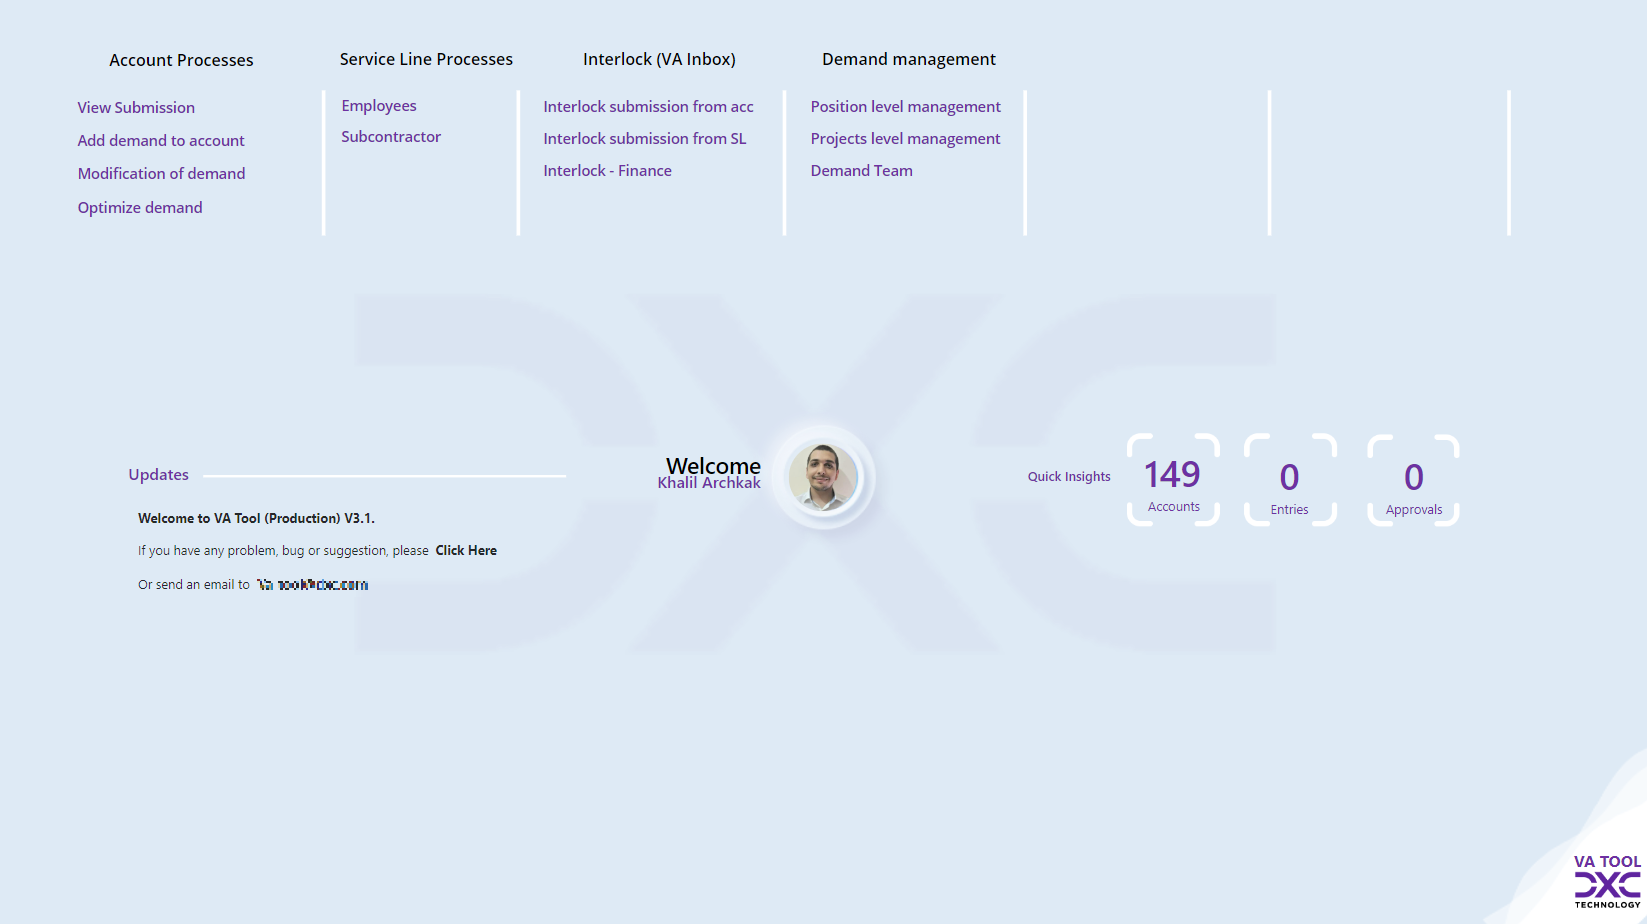
\includegraphics[scale=0.4,keepaspectratio]{Rapport de stage PFE chez DXC/figures/Home_Page.png}
    \caption{Interface d'accueil}
\end{figure}

La page d'accueil regroupe les différentes procédures possibles que propose l'application dans un menu verticale à savoir les procédures en relation avec les comptes, le service line, l'interlock de ces deux dernier mais aussi la gestion des demandes.
\\[0.3cm]
Elle contient aussi un aperçu rapide du nombre de compte affecté pour l'utilisateur, le nombre d'entré saisie par l'utilisateur mais aussi le nombre d'entré validé par ce dernier.
\\[0.3cm]
On peut aussi etre re-directionner vers une application d'aide ou bien envoyer un email en cas de problem a la mailbox de support. 

\newpage
\section{Ajout de masse salariale}
Pour l'ajout de masse salariale au niveau du compte 4 option se presente :

\begin{itemize}
    \item \textbf{Compte existant:} Le compte auxquelle on ajoute une demande existe déja en tant que client
    \item \textbf{New logo:}  Le compte auxquelle on souhaite ajouté une demande n'est pas encore un client
    \item \textbf{Roll-Off\Roll-on:} L'employé qu'on souhaite ajouter se trouve déja dans un autre projet et va changer ce dernier
    \item \textbf{PlaceHolder - add demand:} L'utilisateur souhaite créer une entré pour un future besoin
\end{itemize}

\subsection{Compte existant}

\begin{figure}[!h]
    \centering
    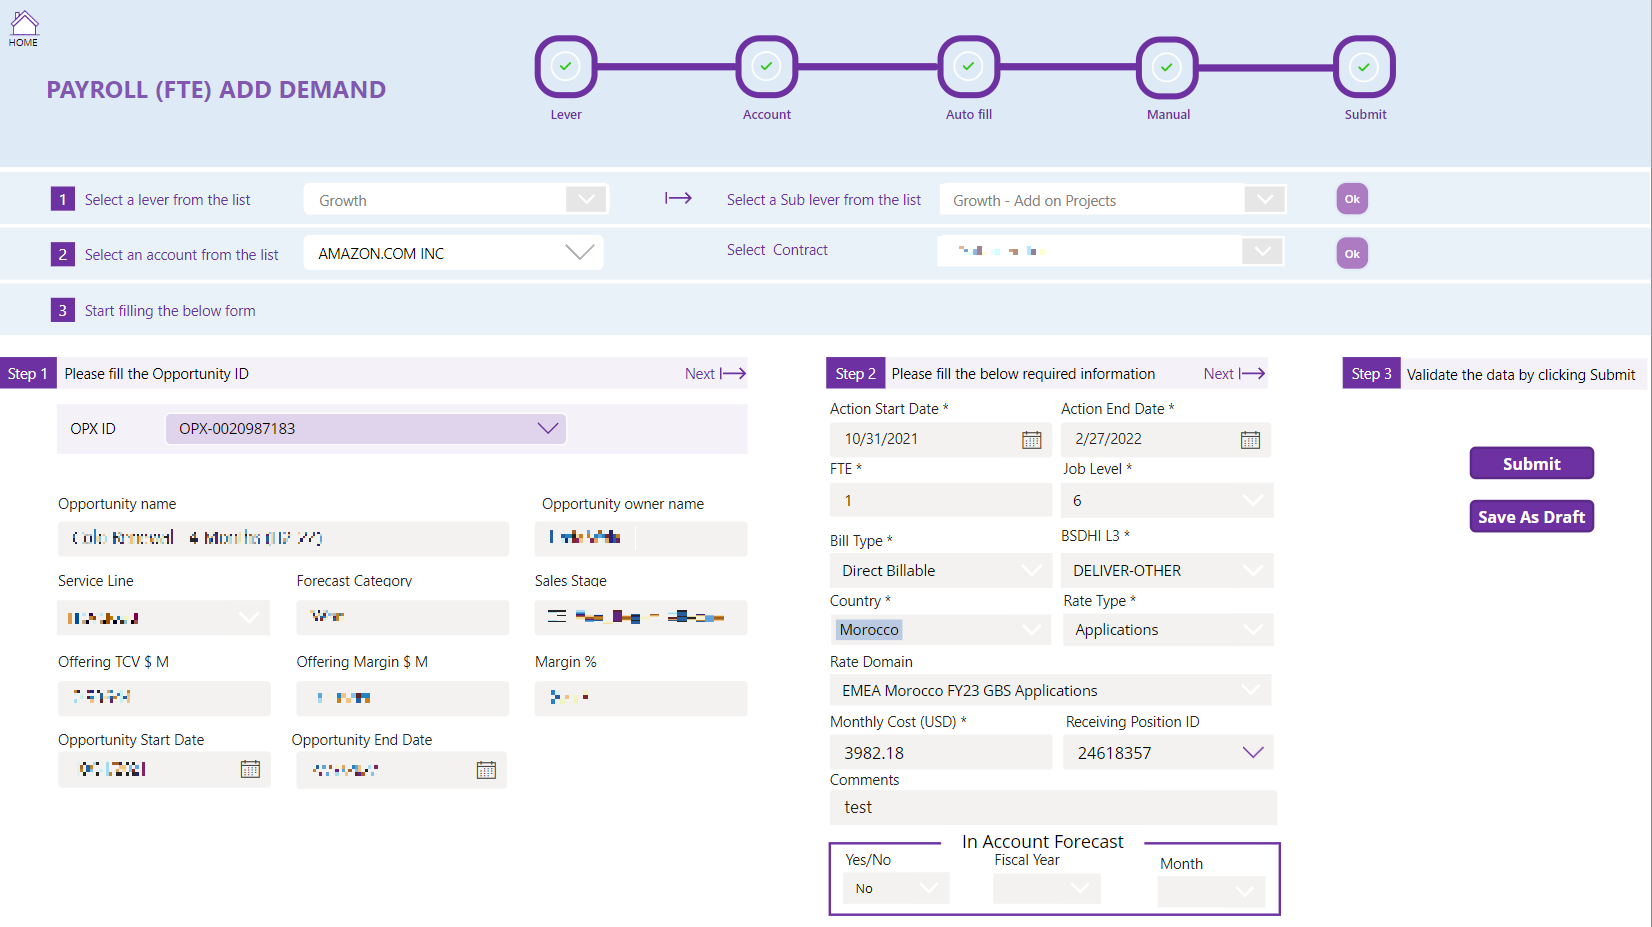
\includegraphics[scale=0.4,keepaspectratio]{Rapport de stage PFE chez DXC/figures/existin_account.png}
    \caption{Ajout de demande - Compte existant}
\end{figure}

L'utilisateur doit sélectionner le compte auxquelles il souhaite ajouter une demande, ensuite il doit saisir l'OPX-ID qui représente un identificateur pour une opportunité, ensuite toutes les informations de la première étape sont automatiquement remplies, puis l'utilisateur doit saisir les différentes informations de la deuxième étape en respectant les différentes contraintes. 
\\[0.3cm]
Deux options s’offrent à l'utilisateur pour saisir l’entrer il peut soit la soumettre directement ou bien l'enregistrer en tant que brouillon pour s'assurer des informations et la soumettre après.

\newpage
\subsection{New Logo}

\begin{figure}[!h]
    \centering
    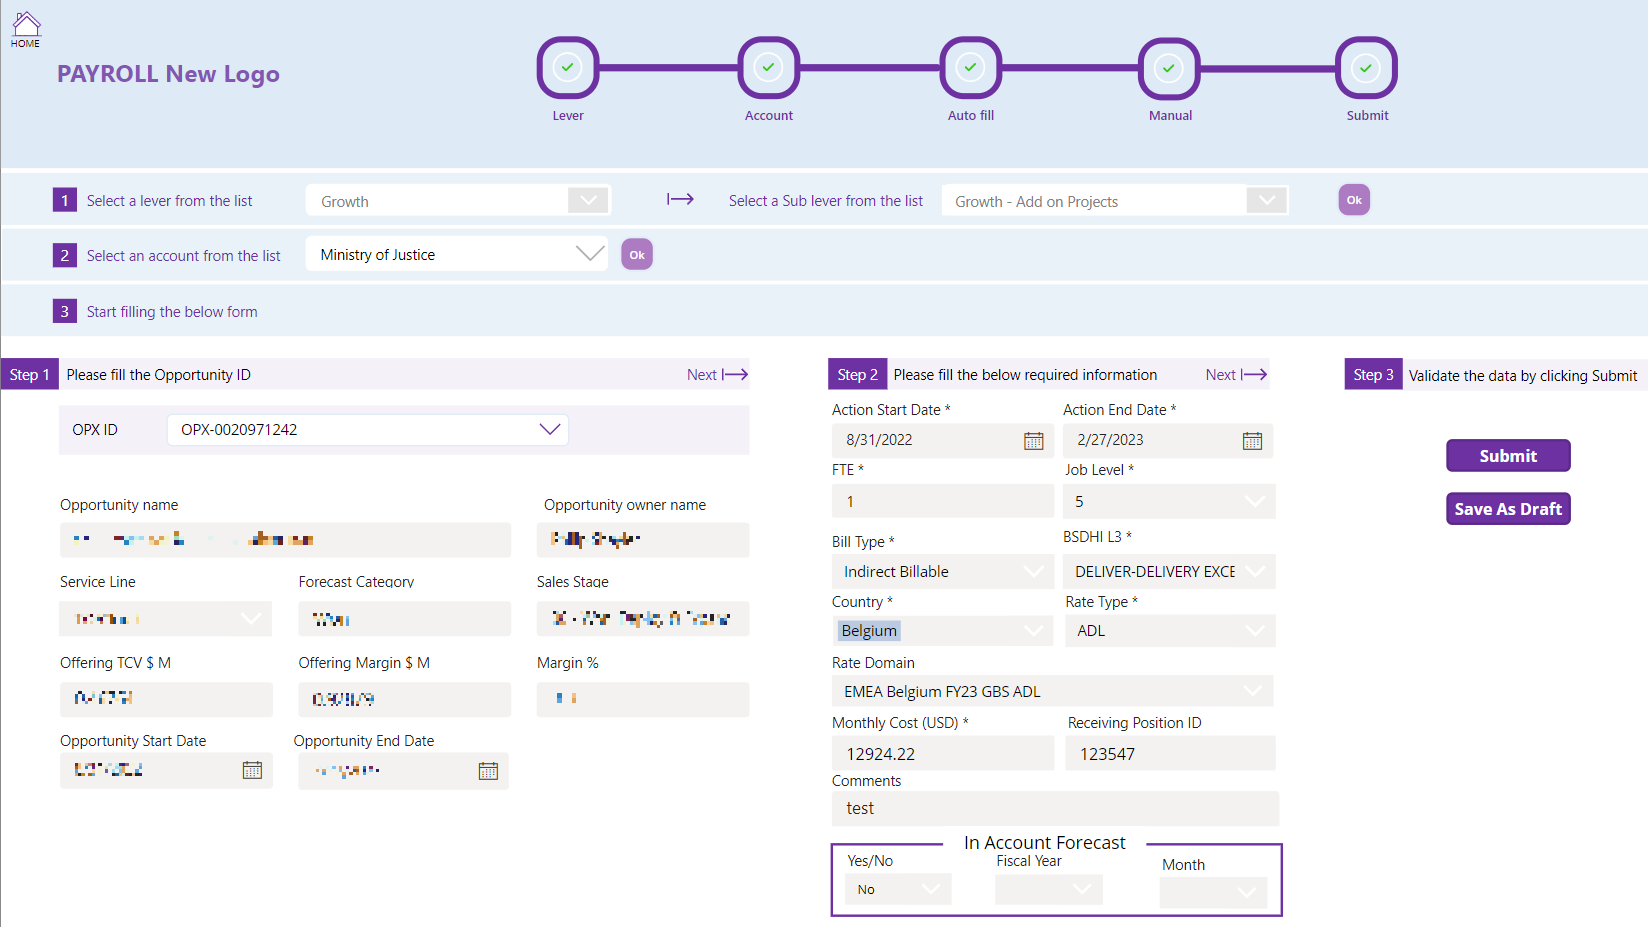
\includegraphics[scale=0.4,keepaspectratio]{Rapport de stage PFE chez DXC/figures/New_Logo.png}
    \caption{Ajout de demande - New Logo}
\end{figure}

Ce formulaire fonctionne de la meme facon que le precedent la seul difference est dans le choix du compte, dans ce dernier le choix du compte est fait a travers le contrat SalesForce car le compte n'est pas encore un client de DXC d'ou le nom de New Logo.

\subsection{Roll-Off / Roll-On}

\begin{figure}[H]
    \centering
    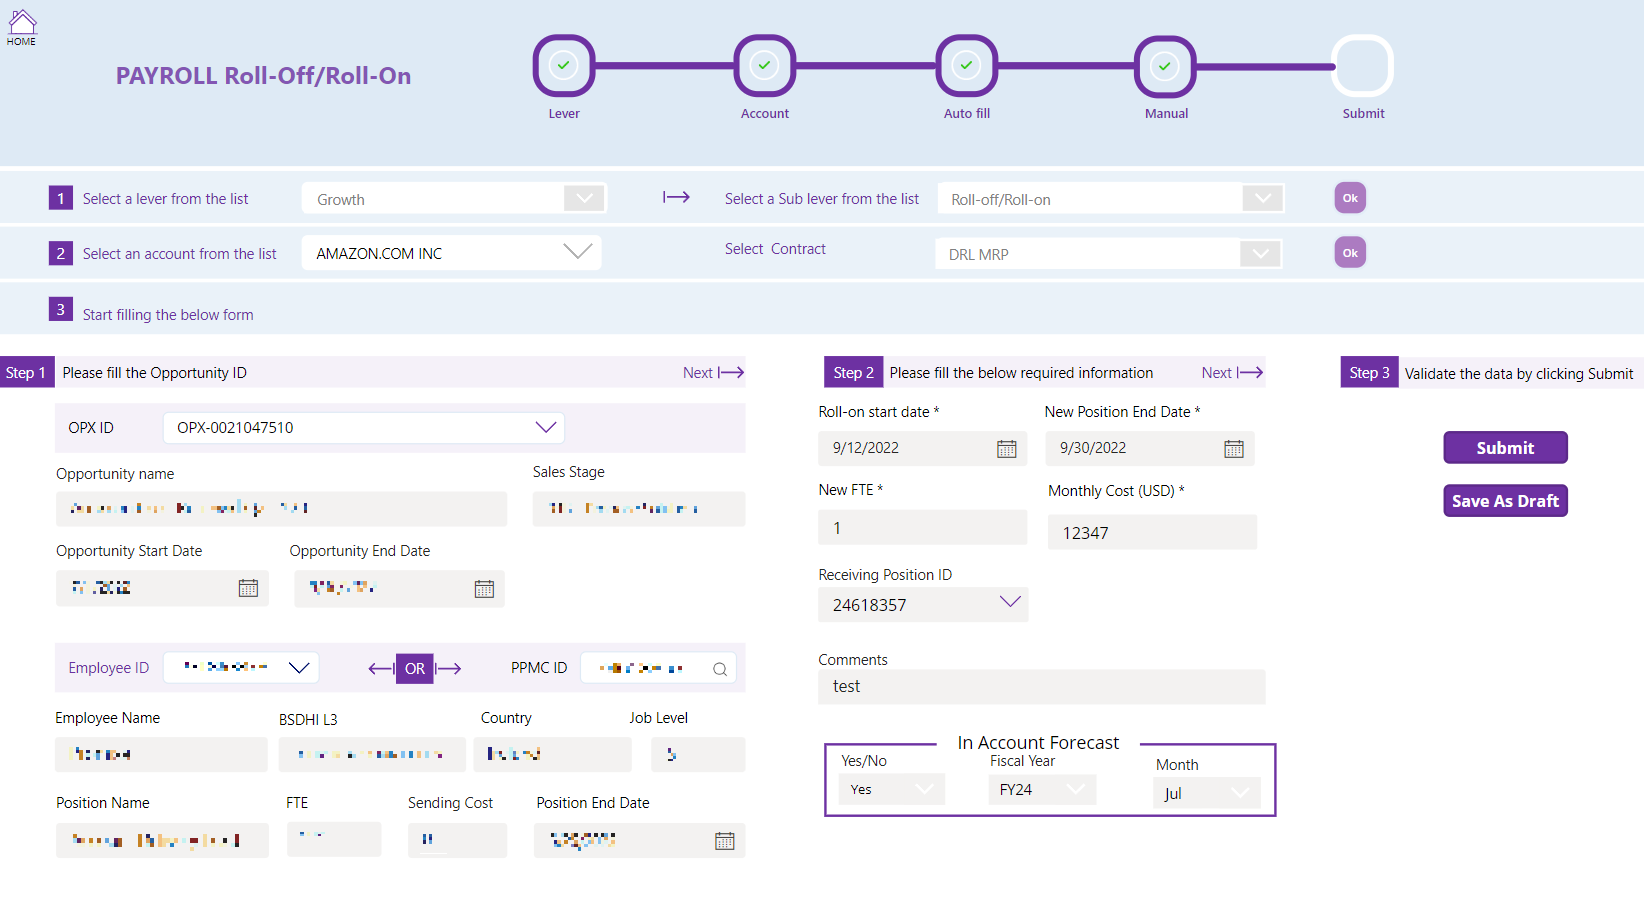
\includegraphics[scale=0.4,keepaspectratio]{Rapport de stage PFE chez DXC/figures/rolloff_rollon.png}
    \caption{Ajout de demande - Roll-Off / Roll-On}
\end{figure}

Pour le "Roll-Off/Roll-On", Un employé change de projet en restant avec le meme client.
\\
Dans la 1er etape l'utilisateur doit saisire l'OPX-ID mais aussi l'identificateur de l'employé qui vas faire la transition, ensuite il remplis les information necessaire dans la deuxieme étape tout en resepectant les differrentes contrainte, ensuite de la meme maniere il peut soit soumettre ou sauvegarder l'entré comme brouillon

\subsection{PlaceHolder - Add Demand}

\begin{figure}[H]
    \centering
    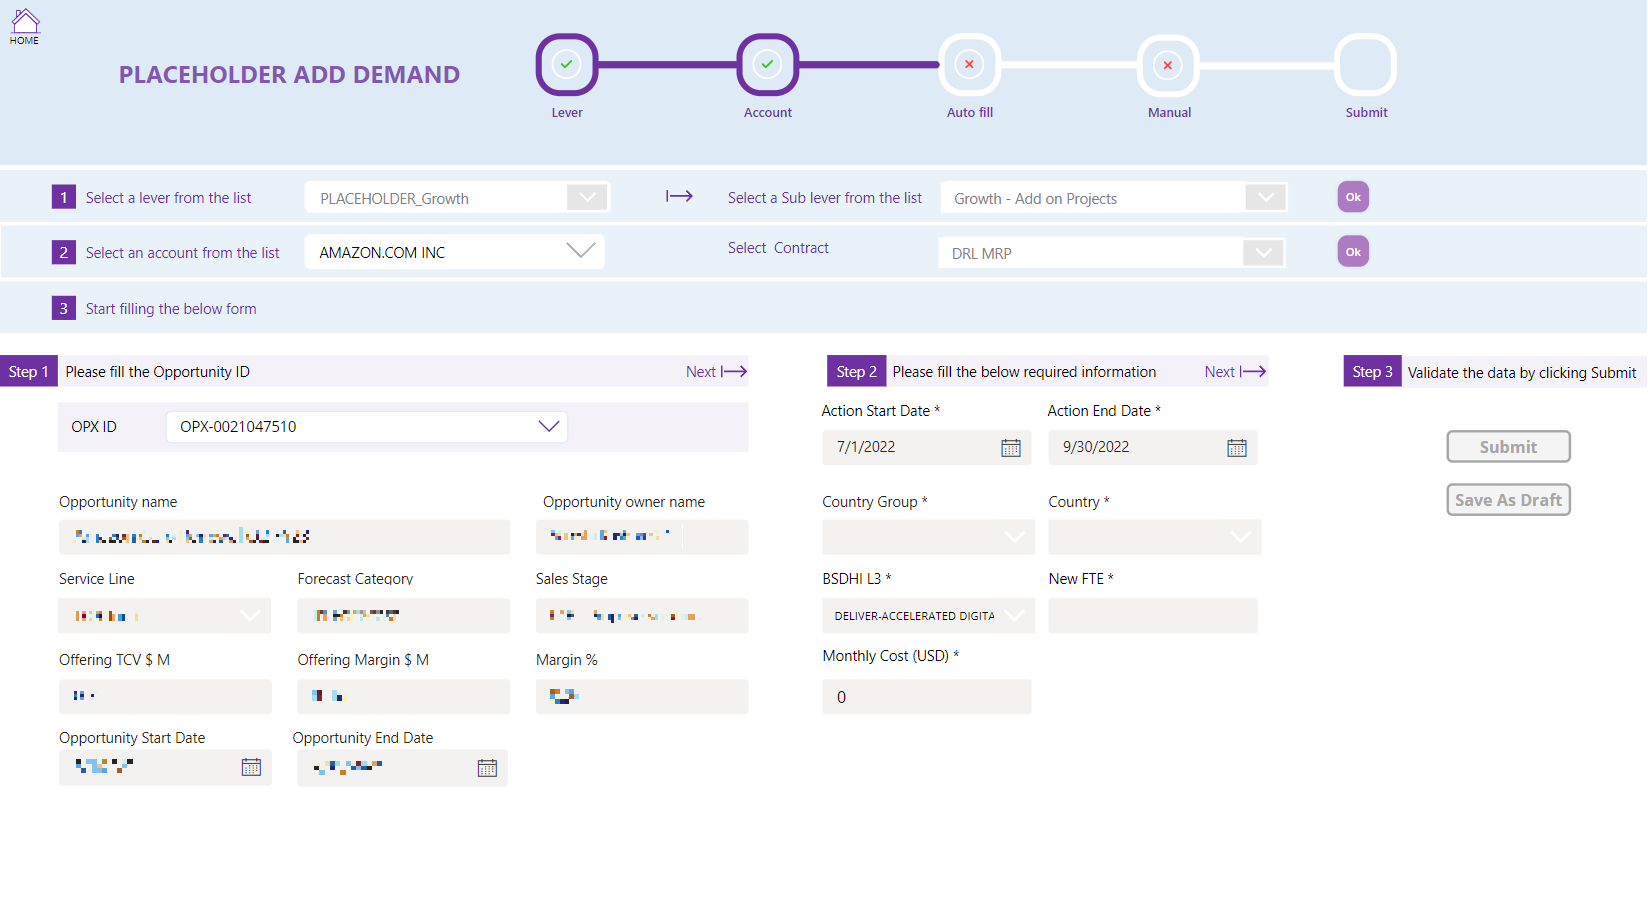
\includegraphics[scale=0.4,keepaspectratio]{Rapport de stage PFE chez DXC/figures/Placeholder_add_demand.png}
    \caption{Ajout de demande - Placeholder Add Demand}
\end{figure}

Pour les placeholders se sont des submission pour un future besoin, aprés avoir créer un placeholder ce dernier peut etre convertis ensuite en une entré VA dans la vue de submission, La soumission de cette entré se fait de la meme maniére que pour l'ajout de demande. 


